\documentclass[11pt]{article}
\usepackage[margin=1in]{geometry}
\usepackage{graphicx}
\usepackage{booktabs}
\usepackage{hyperref}
\usepackage{amsmath}
\usepackage{float}
\usepackage{array}

\title{A reproducible candidate framework for projection-sensitive residual structure in SPARC rotation curves}
\author{Jozsef Olcsak}
\date{2026\\Last revised: 30 August 2026}

\begin{document}
\maketitle

\begin{abstract}
Paper 1 found that externally reviewed structural disturbance is associated with larger low-acceleration residual scatter in SPARC. Paper 2 reversed the question and showed that fixed residual-shape features can recover those A/C labels better than chance, while remaining explicitly non-unique with respect to MOND-simple and empirical RAR-like baselines. This Paper 3 seed asks a narrower follow-up question: where do TPG/projection residuals, MOND-simple residuals, RAR-like residuals, and measured rotation curves point to reproducible projection-sensitive residual candidates? The packet identifies candidate galaxies, radial onset categories, environment/observability stress channels, and a frozen candidate/control ladder anchored by DDO126 and DDO50. A retrospective fixed-packet audit gives one narrow negative result: after a source-only observability and baryonic baseline and the MOND/RAR-common residual descriptor are supplied, the declared projection contrast worsens cross-fitted proper scores under both baselines and all fixed regularization strengths. The unconditioned projection block is itself not stable across that grid. Later EDGE--CALIFA, LITTLE THINGS, and PHANGS routes fail external promotion through negative, mixed, non-specific, source-integrity, or support-gate outcomes. These results constrain their declared finite morphology representations; they neither establish a source-complete body falsification nor permit post-open repair. The paper therefore remains a candidate registry and falsification framework, not conditional-information evidence, physical validation, or gravity-model selection.
\end{abstract}

\section{Purpose and claim boundary}

The working hypothesis is that the TPG/projection baseline may capture part of a local projection-sensitive residual structure, while the remaining TPG residual may carry missing observer- and environment-dependent structure. In this manuscript, ``TPG/projection'' denotes a frozen operational projection baseline used for residual comparison rather than a validated gravity model; TPG is retained as a historical operational label from earlier work and does not imply a validated gravity theory. This is a candidate-search statement, not a validation result. A defensible Paper 3 must therefore separate three layers:
\begin{enumerate}
\item an operational residual layer, based on frozen TPG/projection, MOND-simple, and RAR-like residual maps;
\item a systematics layer, based on distance, inclination, point count, H\,I kinematics, beam smearing, and non-circular motions;
\item an interpretation layer, where any projection-sensitive residual interpretation is allowed only if the residual pattern survives the systematics layer and is more specific than ordinary RAR/MOND behavior.
\end{enumerate}

The permitted claim is that this packet defines a reproducible candidate-selection and control framework for projection-sensitive residual structures. The forbidden claim is that the candidates already validate any physical theory or gravity model.

\section{Data inherited from Papers 1 and 2}

The packet inherits derived SPARC residual artifacts from the Paper 1 and Paper 2 public packages. Raw SPARC rotmod files and raw H\,I survey products are not redistributed. The retained derived tables include pointwise absolute residuals for TPG/projection, MOND-simple, and empirical RAR-like families; galaxy-level residual features; distance, observability, and environment summaries; and small radial-pilot control summaries.

The full Paper 3 reproducibility package, including the candidate/control tables, figures, regeneration script, compiled PDF, and arXiv source package, is archived at \href{https://doi.org/10.5281/zenodo.20285908}{\nolinkurl{doi:10.5281/zenodo.20285908}}. The package can be regenerated with the commands listed in the repository README.

The main residual quantity is
\[
r_{m,gi}=\left|\log V_{{\rm obs},gi}-\log V_{m,gi}\right|,
\]
with galaxy-level burden
\[
{\rm RMS}_{m,g}=\sqrt{{1\over N_g}\sum_i r_{m,gi}^2}.
\]
The TPG-specific excess used for candidate triage is
\[
\Delta_{{\rm TPG-low},g}=
{\rm RMS}_{{\rm TPG},g}-
\min\left({\rm RMS}_{{\rm MOND},g},{\rm RMS}_{{\rm RAR},g}\right).
\]
Positive values mark galaxies where the TPG/projection residual is larger than the best available low-acceleration comparator in this packet. Negative values mark TPG success controls.

\section{Theory motivation}

The relevant external baseline is the SPARC radial acceleration relation \cite{McGaugh2016RAR,Lelli2016SPARC} and the broader MOND/RAR literature \cite{Milgrom1983MOND,Li2018RARFits}. These works are not optional background; they define the strongest ordinary low-acceleration competitor. If a projection-sensitive residual hypothesis only reproduces the same residual ordering as RAR/MOND, it is not yet distinguished.

The systematics literature is equally central. Non-circular motions in H\,I velocity fields \cite{Trachternach2008THINGS,Oman2019NonCircular} and beam-smearing/rotation-curve quality effects \cite{deBlok1997Beam} can generate residual structure without new physics. The JWST/NIRCam Zone-of-Avoidance result \cite{NiloCastellon2025ZoA} is used only as an observer/line-of-sight motivation: foreground obscuration and hidden structure can materially affect what an observer can map. It is not evidence for the projection-sensitive residual interpretation by itself.

\section{Candidate construction}

For each galaxy we record TPG/projection RMS, MOND-simple RMS, RAR-like RMS, TPG-specific excess, environment proxy, distance, reconstruction-risk proxy, inclination, and the first radial bin where the TPG/projection absolute residual exceeds 0.15 dex. Candidate classes are assigned by frozen screening rules:
\begin{itemize}
\item \textit{clean projection-sensitive candidate}: high TPG residual, high TPG-specific excess, and non-high reconstruction risk;
\item \textit{environment-linked projection candidate}: high residual burden with high environment cue;
\item \textit{TPG divergence follow-up}: positive TPG-specific excess without enough cleanliness for the first two labels;
\item \textit{TPG success control}: low residual burden where TPG is no worse than MOND/RAR-like baselines.
\end{itemize}

These classes are triage labels. They are not physical classifications.

\begin{table}[H]
\centering
\caption{Candidate shortlist from the regenerated seed packet.}
\scriptsize
\setlength{\tabcolsep}{3pt}
\begin{tabular}{llrrrp{0.22\linewidth}p{0.18\linewidth}}
\toprule
Galaxy & Class & TPG RMS & TPG excess & Env. & Onset & Candidate class\\
\midrule
UGC00731 & C & 0.340 & 0.093 & 0.00 & inner\_R$<$0.33Rmax & clean projection \\
CamB & A & 0.964 & -0.080 & 1.72 & inner\_R$<$0.33Rmax & environment linked \\
UGC05764 & A & 0.329 & 0.076 & 0.00 & inner\_R$<$0.33Rmax & TPG divergence \\
NGC2403 & A & 0.085 & 0.029 & 1.86 & outer\_R$>$=0.67Rmax & TPG divergence \\
NGC3741 & C & 0.204 & 0.103 & -0.12 & inner\_R$<$0.33Rmax & TPG divergence \\
UGC08490 & C & 0.186 & 0.055 & 0.00 & inner\_R$<$0.33Rmax & TPG divergence \\
NGC3109 & C & 0.176 & 0.039 & 0.20 & middle\_0.33-0.67Rmax & TPG divergence \\
UGC06446 & C & 0.194 & 0.038 & 0.00 & inner\_R$<$0.33Rmax & TPG divergence \\
\bottomrule
\end{tabular}
\end{table}

\section{Residual and environment readouts}

\begin{figure}[H]
\centering
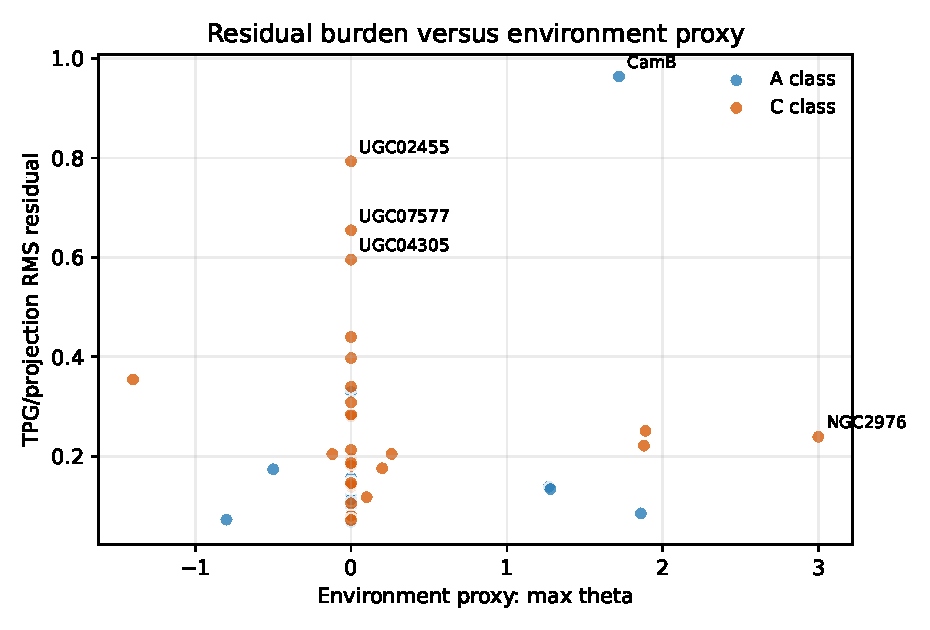
\includegraphics[width=0.82\linewidth]{figures/paper3_environment_residual_scatter.pdf}
\caption{TPG/projection residual burden versus the inherited environment proxy. Named points are the largest seed-candidate scores.}
\end{figure}

\begin{figure}[H]
\centering
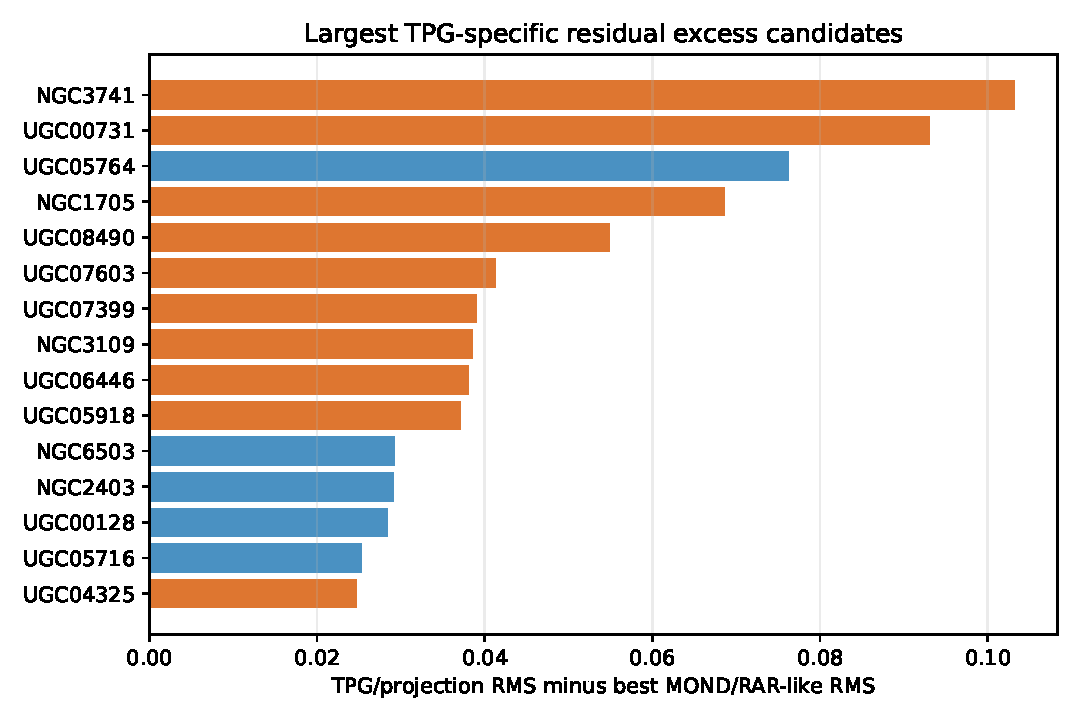
\includegraphics[width=0.82\linewidth]{figures/paper3_tpg_specific_excess.pdf}
\caption{Galaxies with the largest TPG/projection residual excess relative to the better of MOND-simple and RAR-like RMS.}
\end{figure}

\begin{figure}[H]
\centering
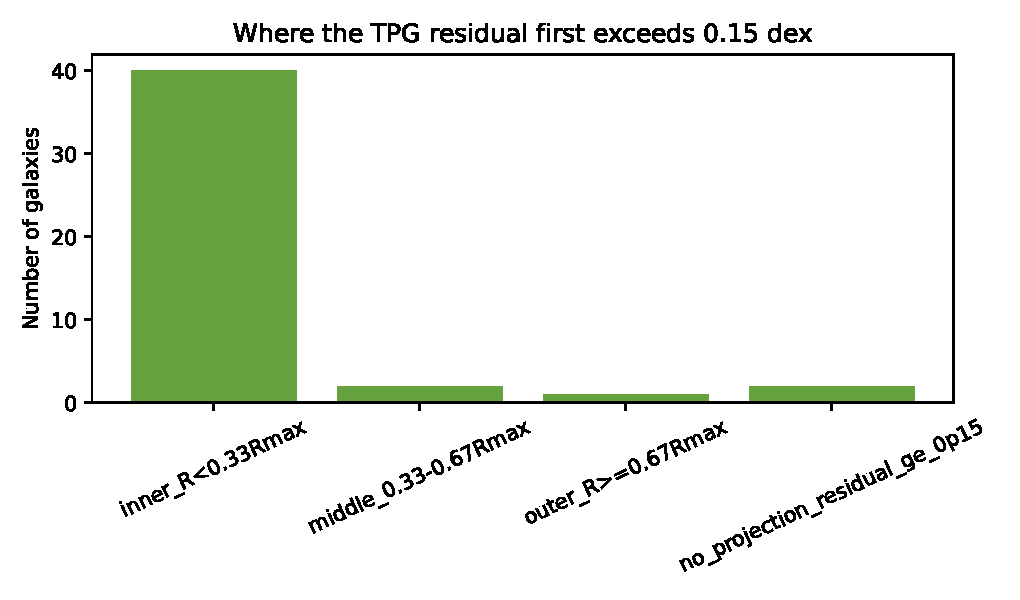
\includegraphics[width=0.78\linewidth]{figures/paper3_residual_onset_bins.pdf}
\caption{Radial bin where the TPG/projection absolute residual first exceeds 0.15 dex. This is a morphology-of-failure diagnostic, not a detection statistic.}
\end{figure}

\begin{table}[H]
\centering
\caption{Screening correlations for TPG/projection residual burden.}
\footnotesize
\begin{tabular}{lrl}
\toprule
Covariate & Pearson $r$ & Interpretation\\
\midrule
DistanceMpc & -0.291 & screening\_correlation\_not\_causal\_attribution \\
EnvMaxTheta & 0.110 & screening\_correlation\_not\_causal\_attribution \\
W\_tau\_eff\_abs\_v01 & 0.983 & screening\_correlation\_not\_causal\_attribution \\
ReconstructionRiskChannel\_v01 & 0.317 & screening\_correlation\_not\_causal\_attribution \\
MeanErrVobsKms & -0.214 & screening\_correlation\_not\_causal\_attribution \\
InclinationErrorDeg & 0.214 & screening\_correlation\_not\_causal\_attribution \\
\bottomrule
\end{tabular}
\end{table}

\begin{figure}[H]
\centering
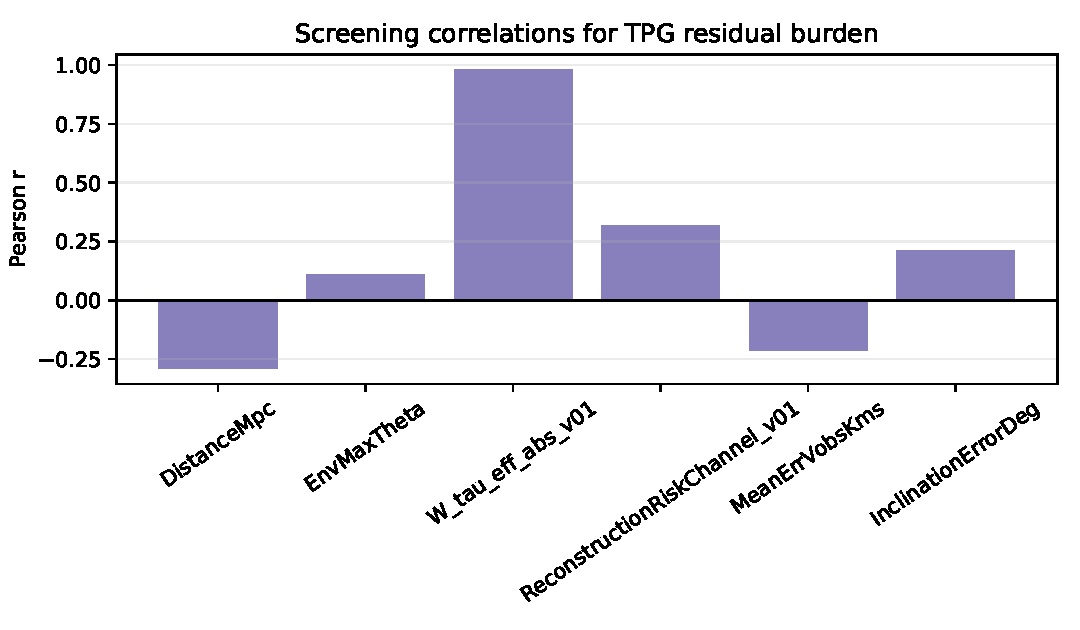
\includegraphics[width=0.82\linewidth]{figures/paper3_observability_stress.pdf}
\caption{Screening correlations with the TPG/projection residual burden. These are not causal estimates.}
\end{figure}

One covariate in this table, W\_tau\_eff\_abs\_v01, is intentionally treated as an internal diagnostic rather than independent evidence. Its correlation with projection residual burden is very high, and the variable is not allowed to support any validation claim until a leakage audit proves that it is not partly defined from the same residual endpoint. In the present manuscript it is therefore a bookkeeping stress term only.

\section{Endpoint-conditioned $S_\tau$ diagnostic}

The descriptive projection-sensitive residual form can be written operationally as
\[
F_\tau(a_N,R)=1+S_\tau(R)\,\alpha\ln\left(1+{a_0\over a_N}\right).
\]
In this section we do not fit a new model. We algebraically invert this expression after substituting the observed-to-baryonic velocity ratio at each radius. For each SPARC point with a usable baryonic baseline, the endpoint-conditioned descriptive value is therefore
\[
S_{\tau,\mathrm{req}}(R)=
{V_{\rm obs}(R)/V_N(R)-1\over \alpha\ln\left(1+a_0/a_N(R)\right)}.
\]
Here $S_{\tau,\mathrm{req}}$ is the value that would be required for the operational form above to absorb the local residual. This is an inverse residual-absorption diagnostic. It is descriptive and endpoint-conditioned. It uses the measured endpoint and therefore is not a predictive field reconstruction, not independent evidence for a physical theory, and not a validation of the projection ansatz. Its role is only to ask what kind of future predictive rule would be needed: a galaxy-level constant, a radial function, an acceleration function, or an environment-coupled function.

\begin{figure}[H]
\centering
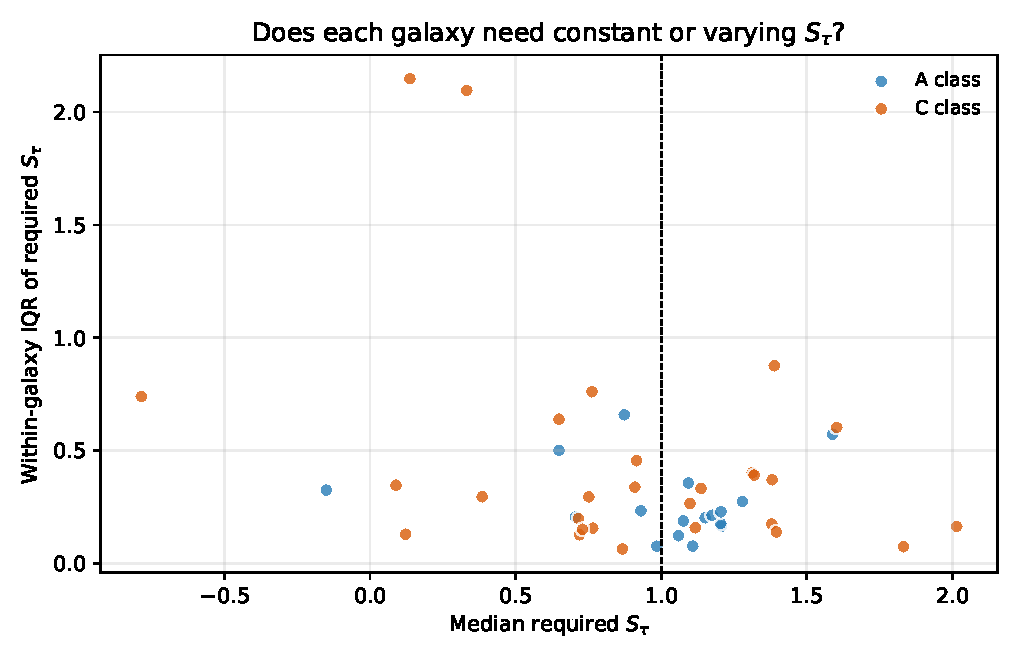
\includegraphics[width=0.78\linewidth]{figures/paper3_required_s_tau_scatter.pdf}
\caption{Median required $S_\tau$ versus within-galaxy spread. A low spread near $S_\tau=1$ would support a constant correction; large spread indicates that a function is needed.}
\end{figure}

\begin{table}[H]
\centering
\caption{In-sample required-$S_\tau$ function-family diagnostics. Lower RMS means that family can absorb the measured TPG residual more compactly.}
\footnotesize
\begin{tabular}{lrrr}
\toprule
Family & Median RMS & Mean RMS & Galaxies\\
\midrule
radius + acceleration & 0.143 & 0.152 & 45 \\
quadratic radius & 0.145 & 0.153 & 45 \\
linear radius & 0.146 & 0.168 & 45 \\
quadratic acceleration & 0.165 & 0.160 & 45 \\
linear acceleration & 0.165 & 0.167 & 45 \\
galaxy constant & 0.187 & 0.183 & 45 \\
fixed S=1 & 0.188 & 0.249 & 45 \\
\bottomrule
\end{tabular}
\end{table}

\begin{figure}[H]
\centering
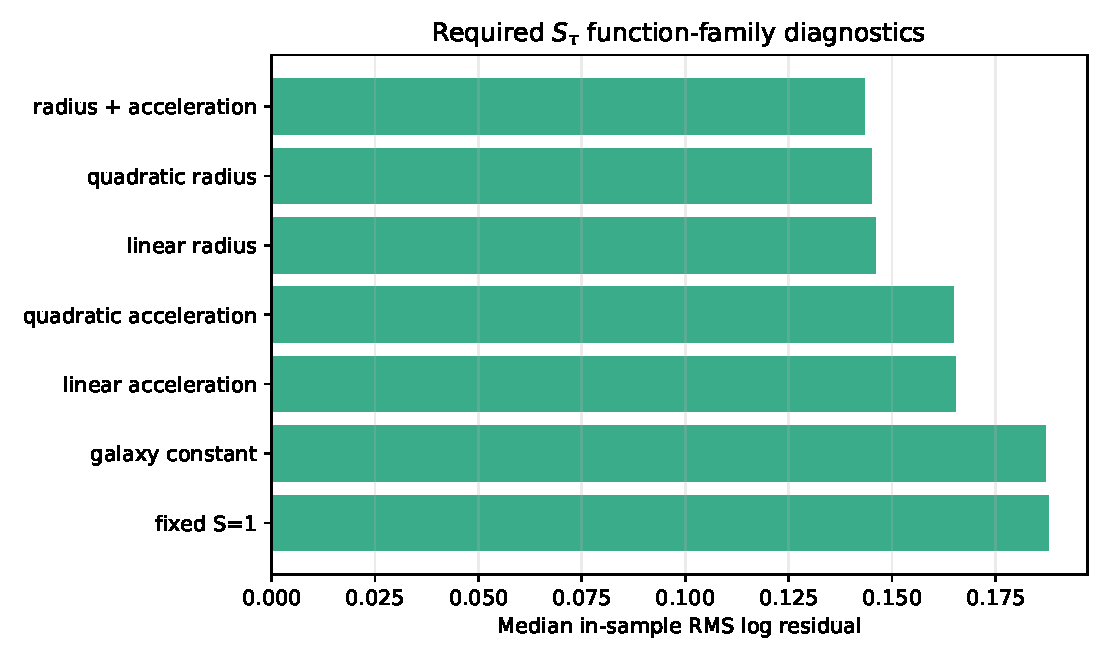
\includegraphics[width=0.82\linewidth]{figures/paper3_s_tau_family_comparison.pdf}
\caption{Diagnostic comparison of constant and simple functional $S_\tau$ families. This is not model selection because the measured velocities are used to infer $S_\tau$.}
\end{figure}

\section{Small-residual controls}

The same diagnostic can be read from the opposite direction. The lowest-quartile TPG/projection RMS objects form a small-residual control set of 12 galaxies, with median projection RMS $0.099854397$ and median required $S_\tau=1.126924435$. These objects ask why the TPG/projection baseline can remain close to the measured curve, rather than why it fails.

The audit gives a cautious answer. One object is classified as a possible local-capture case, where the local TPG/projection baseline may already absorb the dominant local projection-sensitive structure. Three objects are better described as cases where the broader low-acceleration family tracks the measurement well. The remaining eight small-residual objects still carry unresolved radial or external residual structure. Thus good TPG agreement is useful control context, not validation. These rows must remain paired with the high-residual candidates in any future source-native endpoint test.

\section{Heuristic residual-pattern decomposition}

The DDO75/Sextans A stress case motivates a compact heuristic decomposition of the unknown residual pattern. This subsection is not a model-building result and is not used as evidence in the present packet. It is included only to state what a future nonleaky predictor might have to separate. In the working form above, the logarithmic low-acceleration kernel is universal, while the remaining factor $S_\tau(R)$ is allowed to carry source and observer dependence:
\[
S_\tau(R)=S_0
+\beta_{\rm src}C_{\rm src}(R)
+\beta_{\rm path}C_{\rm path}(D)
+\beta_{\rm proj}C_{\rm proj}(B,R_{\max})
+\beta_{\rm drift}C_{\rm drift}(R).
\]
Here $C_{\rm src}$ is source-side radial structure, $C_{\rm path}$ is observer path length or distance, $C_{\rm proj}$ is projection/resolution, and $C_{\rm drift}$ is radial-drift or outer-curve morphology. All four terms are placeholders for future preregistered predictors. None is allowed to use target residuals, required $S_\tau$, or post-hoc endpoint gains as an input.

\section{RMOND comparator status}

RMOND is retained only as a roadmap comparator. The current packet does not contain a frozen pointwise $V_{\rm RMOND}(R)$ law, and therefore it does not contain an RMOND residual endpoint. Local bridge notes show theory-level compatibility and also warn about double counting: at $f_{\rm vec}=0$ the hybrid reduces to the TPG/MTW case, while nonzero vector terms require an independently frozen halo/vector prescription. A future version may add RMOND only after a unique velocity law is preregistered and evaluated on the same SPARC radii as TPG/projection, MOND-simple, and RAR-like baselines.

\section{Post-repair status and next gate}

After the initial seed construction, one repaired branch, DDO168, was rescored under frozen rules as a ladder-consistency example rather than as a primary endpoint. The repaired DDO168 input layer removes the previous mass-closure caveat and gives a single-object specificity-support result: empirical RAR-like remains the best low-acceleration score, but fixed TPG lies within the frozen tie tolerance of the best low-acceleration baseline, with $\Delta_{\rm TPG-best}=0.001509618$ in RMS-log units. The Newtonian baryonic score is worse than fixed TPG by $0.089064802$, and the inverse required-$S_\tau$ diagnostic remains strongly radial, with Pearson $r=0.927628669$.

This result is useful because it places DDO168 beside visible anchors and controls rather than treating it as an isolated success. DDO126 is a positive fixed-TPG public endpoint, DDO50 is a quiet Newtonian-best control with near-zero required-$S_\tau$, DDO154 is a near-one control/countercontrol, and NGC2366 is a caveated lower-amplitude radial candidate. DDO168 therefore strengthens the candidate ladder as a specificity-support example. It is not validation evidence by itself, and it does not select TPG over RAR/MOND as a gravity model.

The paper can now be written as a narrow candidate-registry paper with a frozen local negative result for the declared projection contrast. The eight-object clean endpoint remains a complementary candidate/control branch, but another rescore of the same labels cannot raise the claim. A stronger result requires a source-frozen external matched-tracer endpoint with an explicit common velocity convention and without treating a kinematically selected cohort as independent blind validation.

\section{Post-external-support status}

The later external-support branch adds a useful but deliberately limited result. A preregistered external-only screen is directionally positive: the candidate side has larger endpoint burden than the mandatory controls and countercases under the frozen readout. This supports the idea that the residual candidates are not purely random bookkeeping artifacts. However, the same branch remains observability-caveated. Distance, inclination, point count, H\,I resolution, and source visibility remain possible ordinary explanations, and the external branch cannot substitute for accepted baryonic component data.

For this reason, the current Paper 3 claim is bounded as follows. The manuscript may report a coherent candidate-support pattern in residual and external-proxy diagnostics. It may also report that a future external-plus-component readout has been frozen as a nonexecuted contract. It may not claim that a physical theory has been validated, that TPG has been selected over MOND/RAR, or that the missing source-native component endpoint has been satisfied.

The frozen combined contract compares three future predictors only after accepted component inputs pass intake: an external-only predictor, a component-only predictor, and an external-plus-component predictor. Endpoint outputs and diagnostics such as Vobs residuals, FunctionGain, ProjectionRMS\_TPG, and required $S_\tau$ are forbidden as predictor inputs. This keeps the validation route alive without allowing endpoint-driven retuning.

\section{Anchor/control rotation curves}

Figure~\ref{fig:anchor-control-rotation} shows the two most important current visual endpoints. DDO126 is the positive public-only anchor candidate, and DDO50 is the required control. The panels are diagnostic visualizations of the frozen candidate/control ladder. They are not independent validation and they do not replace the component-input gate.

\begin{figure}[ht]
\centering
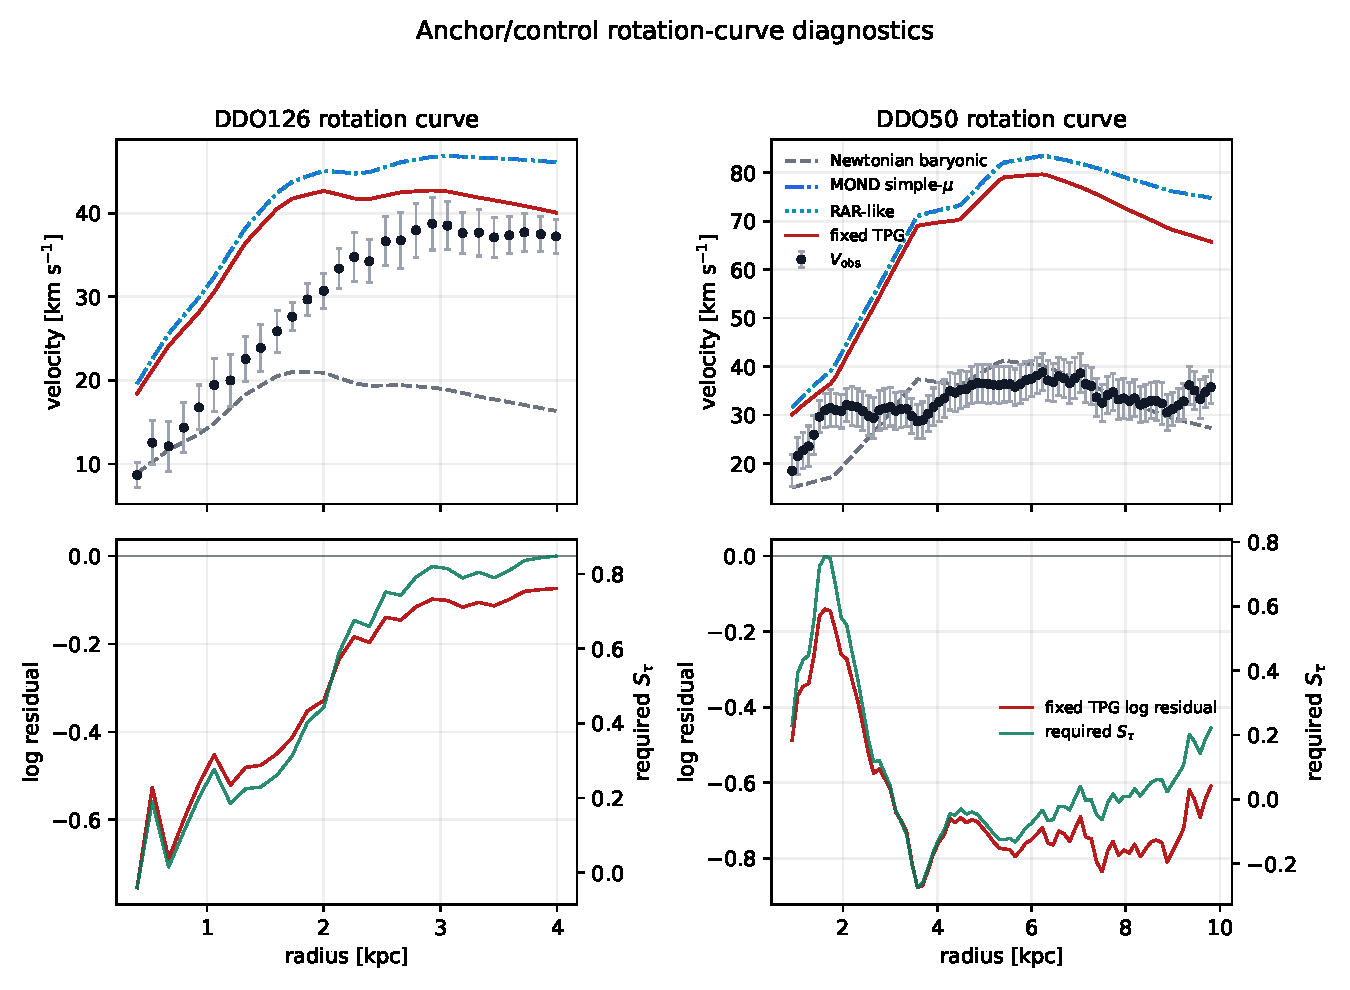
\includegraphics[width=0.94\linewidth]{figures/paper3_anchor_control_rotation_curves.pdf}
\caption{Anchor/control rotation-curve diagnostics. Top panels compare observed rotation speeds with the frozen Newtonian baryonic, MOND-simple, empirical RAR-like, and fixed-TPG curves. Bottom panels show the fixed-TPG log residual and the inverse required-$S_\tau$ diagnostic. The figure is a visual check on the candidate/control ladder, not a validation endpoint.}
\label{fig:anchor-control-rotation}
\end{figure}

\section{Current candidate-ladder status}

The later DDO126/DDO50 and held-out readiness audits sharpen the current claim boundary. The manuscript can report a reproducible candidate ladder with named positive anchors, mandatory controls, and failure-mode objects. DDO126 is the strongest public-only positive anchor candidate in the present packet, while DDO50 is the required control branch. WLM is retained as a geometry/observability stress context. NGC2366 remains caveated radial support and must be reported with DDO154 as its countercontrol. IC1613 and DDO47 remain sensitivity and failure-mode objects until their stellar or component-input blockers are repaired.

This status does not add a new endpoint score. It is a claim-control layer. The input watchlist defines what would be needed for a future upgrade: schema-clean component intake for DDO126/DDO50, or a broader component-confirmed held-out pool. Any new file must pass provenance, column-schema, unit/radius, geometry/systematics, and control-visibility checks before model scores are rerun.

Therefore the current paper-level claim is bounded but nontrivial. The packet records a reproducible operational candidate/control ladder and freezes the component-intake route required to test it. The result is not a physical validation, not gravity-model selection, and not evidence that the residual pattern is unique to a projection-sensitive interpretation. Additional scoring without new accepted component, stellar, or external matched-tracer inputs is not a claim-upgrade path.

The inverse required-$S_\tau$ and related correction curves are effective terminal discrepancies.  They do not uniquely reconstruct a force law, a clock distortion, a spatial-metric distortion, or a full observer-source coframe.  The later companion full-4D descent therefore changes the interpretation but not the numerical candidate ladder: a new 4D endpoint may be scored only after a radial relative coframe and its photon-transfer map are derived and frozen independently of the target residual.  The exact inherited score must use the complete standard excess $E_K=(K_{HH}-K_{\rm std})-CK_{VV}^{-1}C^\dagger$, not the positive Schur term alone, and must retain the full covariance of all jointly scored terminal images.  The present candidate ladder supplies none of those frozen physical inputs.

\section{Retrospective projection-contrast audit}

The original residual association is an unconditional prevalidation result. We therefore added a stricter retrospective audit on the same frozen 45-galaxy A/C sample. The baseline contains seven endpoint-free observability variables: distance, fractional distance error, inclination, inclination error, point count, mean velocity uncertainty, and angular radial coverage. A second baseline adds seven source-side baryonic or morphology summaries derived from the public SPARC component tables without using $V_{\rm obs}$: Hubble type, median baryonic speed, gas and bulge fractions, median disk surface brightness, and two radial-shape ratios. Every raw component file is represented by a SHA-256 hash in the derived source packet.

For each residual family we use the same five-dimensional block: RMS, outer/inner ratio, radius correlation, low-acceleration mean, and fraction above the fixed 0.15 threshold. Predictions are produced by repeated stratified five-fold cross-validation. Three regularization strengths, $C\in\{0.03,0.3,3\}$, are reported without selecting the best one. The key specificity comparison first supplies the MOND/RAR-common descriptor
\[
Z_{\rm std}={1\over2}(Z_{\rm MOND}+Z_{\rm RAR})
\]
and then asks whether the projection contrast
\[
Z_{\rm proj\perp}=Z_{\rm projection}-Z_{\rm std}
\]
improves held-out prediction. This is an operational de-overlap test: naming three residual families does not make them independent information channels.

At $C=0.3$, the observability-plus-baryonic baseline has cross-fitted AUC 0.874. Adding $Z_{\rm proj\perp}$ after $Z_{\rm std}$ changes AUC by -0.019, changes log-loss improvement by -0.040, and changes Brier improvement by -0.012, where positive proper-score differences would favor the enlarged model. Both proper scores therefore worsen. More importantly, the declared contrast comparison worsens both proper scores under both baselines and all three fixed regularization strengths. The generic projection block shows a small improvement only under the strongest shrinkage and fails stability across the grid. Because the directional gate failed, no one-sided positive-increment permutation claim was opened. The packet verdict is therefore a failure of the declared projection-contrast increment in this frozen A/C packet, not a universal no-information verdict.

This audit does not prove that rotation residuals contain no additional information. It shows only that the declared projection contrast does not isolate a stable positive increment in this 45-galaxy label experiment once the source/observability packet and common MOND/RAR residual structure are retained. The generic projection block has positive proper-score increments at the strongest shrinkage, so the result cannot be promoted to an absence claim for projection information in general. The A/C labels also remain within the same broad H\,I/kinematic observational ecosystem and are not an independent survey-level replication.

A later Paper 8 endpoint completed the source-frozen EDGE--CALIFA route using seven untouched confirmatory galaxies after source-only development. The matched-minus-wrong contrast was $\overline D=-0.0586793$, with median $+0.110202$, four of seven positive galaxies, and exact one-sided $p=0.6015625$. All declared max-$T$ controls also failed. An independent implementation rebuilt all 140 terminal coefficients from the common-grid database \cite{Wong2024EDGEDatabase} to a maximum absolute difference of $3.553\times10^{-15}\,{\rm km\,s^{-1}}$. This is a reproducible negative for the declared morphology-alignment proxy, not an independent Tau-specific test or a direct reproduction of the published 17-galaxy kinematic subsample \cite{Levy2018EDGEKinematics}.

The subsequent public-data ladder remains non-promotable. LITTLE THINGS \cite{Oh2015LITTLETHINGS} transfers one frozen scale-tail family to 14 galaxies and 313 points; it improves mean RMSE over TPG/v6 by only $0.101\,{\rm km\,s^{-1}}$ and is $0.649\,{\rm km\,s^{-1}}$ worse than MOND. In PHANGS \cite{Lang2020PHANGSKinematics,Emsellem2022PHANGSMUSE,Querejeta2021PHANGSStructures}, a three-galaxy low-order differential route is null ($p=0.8082$); a two-galaxy $m=2$ route is non-specific because its $m=1$ control is also non-null and the source-label audit fails; and a four-galaxy radial-body confirmation stops at its predeclared 12-sector occupancy gate before any score is released. NGC4254 retains an internally controlled source-coordinate candidate, but a free terminal gain exactly saturates the scalar endpoint and the primitive gain remains non-identifiable.

\section{Predictive validation gate}

The present manuscript is not a validation paper, but it does more than list curiosities. It defines where a projection-sensitive residual signal should be looked for, which controls must travel with the candidates, and what predictor inputs are forbidden. The retrospective audit above is not the missing prospective rule and it failed only the declared contrast-increment gate in the frozen A/C packet. A validation-oriented version must pass a stricter independent gate before any discovery language is appropriate.

First, the residual-pattern rule must be frozen before reading the endpoint residuals. The rule may use source-side structure, distance or line-of-sight information, projection/observability quantities, and preregistered radial-shape information, but it may not use Vobs residuals, FunctionGain, ProjectionRMS\_TPG, or the inverse required-$S_\tau$ diagnostic as predictor inputs. Second, the rule must be evaluated on a predeclared clean candidate/control set, including both positive anchors and controls. Third, the result must improve the frozen endpoint relative to TPG/projection, MOND-simple, and empirical RAR-like baselines, not merely reproduce a generic low-acceleration ordering. Fourth, the improvement must survive the ordinary observability nulls: distance, inclination, point count, beam smearing, H\,I resolution, and non-circular motion.

This predictive gate is the main upgrade path from a seed paper to a validation paper. In practical terms, the next claim-raising experiment is: freeze a predictive projection-sensitive residual rule, then test whether it improves the predeclared clean candidate/control set beyond TPG/projection, MOND-simple, and RAR-like baselines. Until that experiment is passed, the correct status is candidate-support methodology rather than physical evidence.

The morphology representation itself is now part of that freeze. Let $\Phi_k$ be the finite source record and $T_k$ the complete body--channel--observer-resolution--terminal map. A terminal rule can factor as $T_k=f_k\circ\Phi_k$ only if $T_k$ is constant on every $\Phi_k$ fibre. A failure can therefore expose an imprecise or lossy $\Phi_k$ without falsifying every richer body representation. This qualification has a strict anti-leakage partner: after endpoint $y$ is known, adding $y$ to the source span forces its projected residual to zero. Accordingly, a refined $\Phi_{k+1}$ must be derived from source-only information and tested on a new untouched packet; the opened SPARC, EDGE--CALIFA, LITTLE THINGS, and PHANGS packets cannot be repaired into confirmation.

\section{Interpretation}

The most useful interpretation is modest. TPG success controls show where the local projection baseline is already adequate. TPG divergence follow-ups show where the residual has structure that might encode missing observer/environment-sensitive information, but these are exactly the cases where ordinary systematics can also enter. A candidate becomes interesting only when three facts hold together: the TPG residual diverges in a structured radial way, the divergence is not shared by all low-acceleration baselines, and the object has a plausible projection-sensitive residual pattern that is not reducible to distance, inclination, beam smearing, or non-circular motion.

% BEGIN OBSERVER UPDATE 20260914
\section{Observer realization: inherited results and physical boundary}
\label{sec:observer-update-20260914}
The current observer programme distinguishes a conditional mathematical
construction from an occupied physical measuring system. The source order
remains base plus one universal seed, stabilized morphological response,
observer--source restriction, shared descriptor, and resolved terminal
readouts. Neither a detector nor an empirical residual constructs the parent
body backwards. Dynamics below concern downstream subsystems only.

The canonical observer-origin derivation, Sections 22--26, owns the following
results. The existing joint source action fixes static and frequency-dependent
response together. Variation of the BRAC potential couples to the field
square; a linear field coupling is a distinct comparator unless derived by
expansion about an occupied background. Fixed canonical means select a unique
coherent state in a finite positive harmonic packet only if there is no excess
fluctuation energy. This is a free/asymptotic preparation statement, not the
ground state of an interacting detector. For the existing coupled harmonic
pair, the joint ground is pure but either local subsystem is mixed, with its
covariance fixed by the complete joint Hamiltonian.

These are conditional derivations and internal numerical checks. The actual
observer--source context, physical preparation process, kinetic/energy
calibration and stable operational resolution remain unproved. The existing
ORA-T1 selector conditionally chooses stable quantizers when the occupied
context, admissible partition family and positive closure barrier are supplied;
it does not establish those physical premises. A computed ground state is not
a preparation mechanism, and a covariance or optimal abstract measurement is
not an implemented stable quantizer $Q_{OS}$.

\paragraph{Ownership and use.}
The central observer-origin note owns the new contact, state and covariance
derivations; the body-readout technical companion carries the consolidated
mathematics. Foundation Papers IV, V and VI retain physical-selection,
clock-descent and quantum-readout ownership, respectively. This paper imports
only the consequences within its scope. No observational dataset, baseline,
frozen coefficient, score or empirical conclusion is revised by this update.
The reproducibility supplement records the source hashes and the exact
conditional/physical distinction.


\paragraph{Consequence for this paper.}
For galactic inference, these observer constructions do not derive a rotation-curve correction or identify a measured residual as a parent effect. Existing endpoint freezes and scores are unchanged.
% END OBSERVER UPDATE 20260914

% BEGIN STATE UPDATE 20260918
\section{Source identification and recovery}
The current observer audit separates a conditional forward construction from physical source selection. A frozen body, occupied observer incidence, preparation, complete instrument and stable resolution can determine records without selecting those inputs from Nature. Equal effects do not fix postmeasurement states, and symmetry within a chosen interaction family does not exclude other symmetric couplings. For galactic inference, these observer constructions do not derive a rotation-curve correction or identify a measured residual as a parent effect. Existing endpoint freezes and scores are unchanged.

\paragraph{Dependency and claim ownership.}
Foundation VI and the body--readout technical companion own the finite instrument/access proof; Foundation IV and TD-0 retain physical source selection; Foundation V, the temporal synthesis and seed--body companion own the gradient/inertial distinction. This paper inherits only the stated specialization. Canonical assumptions, countermodels and calibration audits are in \url{https://github.com/tau-core-research/tau-core-theory/blob/main/docs/tau_rqm_instrument_to_record_bridge_001.md}. No physical seed, Nature occupation or Tau-exclusive observation is established by this update. Existing empirical endpoint definitions and scores are unchanged.
% END STATE UPDATE 20260918

% BEGIN PAIR READOUT UPDATE 20260927
\section{Conditional source preparation and time-resolved access}
The common-operator scalar--Dirac completion now supports an explicit
conditional chain from interaction vertices to pair transfer and joint
readout. Nonzero vertices do not select occupation. Relational coherence
can be generated from an occupied number-diagonal pair even while both
local mean fields vanish. In a declared resonant rotating-wave and Markov
loss model, finite-window emission retains this coherence information,
whereas an all-time count discards it. This is standard-compatible quantum
recovery, not a Tau-specific observational residual.
For galactic inference, these observer constructions do not derive a rotation-curve correction or identify a measured residual as a parent effect. Existing endpoint freezes and scores are unchanged.
\paragraph{Dependency ownership and limits.}
The P4 common-source assembly owns the scalar/Yukawa benchmark and finite
preparation calculations; Foundation VI and the body--readout companion
inherit the joint-access mathematics. Foundation IV and TD-0 retain
physical source selection, and Foundation V retains clock descent.
The parent remains atemporal: the evolution above is a conditional
downstream 4D model, not parent memory or a derived morphogenetic time.
Physical initial occupation, a gauge-complete realization, detector
amplification, absolute calibration and stable observer-relative $Q_{OS}$
remain unselected. No empirical endpoint or score is changed.
The canonical derivation and reproducible numerical sources are linked at
\url{https://github.com/tau-core-research/tau-core-theory/blob/main/docs/tau_core_p4_nonabelian_particle_common_source_assembly_001.md}.
% END PAIR READOUT UPDATE 20260927

\section{Conclusion}

This paper establishes a reproducible candidate-search framework rather than merely proposing one. It carries forward the discipline learned from Papers 1 and 2: freeze the endpoint, compare against MOND/RAR baselines, name the systematics, and avoid promoting a diagnostic pattern into physical evidence. The repaired DDO168 branch, the external-support branch, and the DDO126/DDO50 candidate-ladder lock organize the residual candidates into a falsifiable target set. The retrospective audit adds a narrow negative result: the declared projection contrast supplies no stable positive predictive increment in the frozen 45-galaxy A/C packet. It does not establish that all projection-sensitive rotation information is absent.

The EDGE--CALIFA, LITTLE THINGS and PHANGS continuations have now been run far enough to show that none raises the claim under its frozen gate. The next claim-raising step is therefore not a re-analysis of those opened packets. It is a source-frozen, signed, unit-calibrated forward prediction from a richer endpoint-blind morphology representation, evaluated in a new independent survey or release with a complete standard comparator and predefined observability controls. Only after that gate can the paper ask whether the residual candidates are truly projection-sensitive rather than ordinary low-acceleration or H\,I-systematics behavior.

\bibliographystyle{plain}
\bibliography{references}

\end{document}
